\appendix

\section{Equivalence of transitive closure definitions}\label{def_eq}

To show the equivalence of $a^{cf}$ and $a^+$ definitions of transitive closure, we introduce the partial order $\succeq$ on matrices with fixed size that have subsets of $N$ as elements. For square matrices $a, b$ of the same size we denote $a \succeq b$ iff $a_{i,j} \supseteq b_{i,j}$, for every $i, j$. For these two definitions of transitive closure, the following lemmas and theorem hold.

\begin{lemma}\label{lemma:cf_geq_valiant}
	Let $G =(N,\Sigma,P,S)$ be a context-free grammar in Chomsky Normal Form, let $a$ be a square matrix. Then $a^{(k)} \succeq a^{(k)}_+$ for any $k \geq 1$.
\end{lemma}
\begin{proof}(Proof by Induction)
	
	\textbf{Basis}: The statement of the lemma holds for $k = 1$, since $$a^{(1)} = a^{(1)}_+ = a.$$
	
	\textbf{Inductive step}: Assume that the statement of the lemma holds for any $k \leq (p - 1)$ and show that it also holds for $k = p$ where $p \geq 2$. For any $i \geq 2$ $$a^{(i)} = a^{(i-1)} \cup (a^{(i-1)} \times a^{(i-1)}) \Rightarrow a^{(i)} \succeq a^{(i-1)}.$$ Hence, by the inductive hypothesis, for any $i \leq (p-1)$ $$a^{(p-1)} \succeq a^{(i)} \succeq a^{(i)}_+.$$ Let $1 \leq j \leq (p - 1)$. The following holds $$(a^{(p-1)} \times a^{(p-1)}) \succeq (a^{(j)}_+ \times a^{(p-j)}_+),$$ since $a^{(p-1)} \succeq a^{(j)}_+$ and $a^{(p-1)} \succeq a^{(p-j)}_+$. By the definition, $$a^{(p)}_+ = \bigcup^{p-1}_{j=1}{a^{(j)}_+ \times a^{(p-j)}_+}$$ and from this it follows that $$(a^{(p-1)} \times a^{(p-1)}) \succeq a^{(p)}_+.$$ By the definition, $$a^{(p)} = a^{(p-1)} \cup (a^{(p-1)} \times a^{(p-1)}) \Rightarrow a^{(p)} \succeq (a^{(p-1)} \times a^{(p-1)}) \succeq a^{(p)}_+$$ and this completes the proof of the lemma.
\end{proof}

\begin{lemma}\label{lemma:valiant_geq_cf}
	Let $G =(N,\Sigma,P, S)$ be a context-free grammar in Chomsky Normal Form, let $a$ be a square matrix. Then for any $k \geq 1$ there is $j \geq 1$, such that $(\bigcup^{j}_{i=1}{a^{(i)}_+}) \succeq a^{(k)}$.
\end{lemma}
\begin{proof}(Proof by Induction)
	
	\textbf{Basis}: For $k = 1$ there is $j = 1$, such that $$a^{(1)}_+ = a^{(1)} = a.$$ Thus, the statement of the lemma holds for $k = 1$.
	
	\textbf{Inductive step}: Assume that the statement of the lemma holds for any $k \leq (p - 1)$ and show that it also holds for $k = p$ where $p \geq 2$. By the inductive hypothesis, there is $j \geq 1$, such that $$(\bigcup^{j}_{i=1}{a^{(i)}_+}) \succeq a^{(p-1)}.$$ By the definition, $$a^{(2j)}_+ = \bigcup^{2j-1}_{i=1}{a^{(i)}_+ \times a^{(2j-i)}_+}$$ and from this it follows that $$(\bigcup^{2j}_{i=1}{a^{(i)}_+}) \succeq (\bigcup^{j}_{i=1}{a^{(i)}_+}) \times (\bigcup^{j}_{i=1}{a^{(i)}_+}) \succeq (a^{(p-1)} \times a^{(p-1)}).$$ The following holds $$(\bigcup^{2j}_{i=1}{a^{(i)}_+}) \succeq a^{(p)} = a^{(p-1)} \cup (a^{(p-1)} \times a^{(p-1)}),$$ since $$(\bigcup^{2j}_{i=1}{a^{(i)}_+}) \succeq (\bigcup^{j}_{i=1}{a^{(i)}_+}) \succeq a^{(p-1)}$$ and $$(\bigcup^{2j}_{i=1}{a^{(i)}_+}) \succeq (a^{(p-1)} \times a^{(p-1)}).$$ Therefore there is $2j$, such that $$(\bigcup^{2j}_{i=1}{a^{(i)}_+}) \succeq a^{(p)}$$ and this completes the proof of the lemma.	
\end{proof}

\begin{mytheorem}\label{thm:closures}
	Let $G =(N,\Sigma,P,S)$ be a context-free grammar in Chomsky Normal Form, let $a$ be a square matrix. Then $a^+ = a^{cf}$.
\end{mytheorem}
\begin{proof}
	
	By the lemma~\ref{lemma:cf_geq_valiant}, for any $k \geq 1$, $a^{(k)} \succeq a^{(k)}_+$. Therefore $$a^{cf} = a^{(1)} \cup a^{(2)} \cup \cdots \succeq a^{(1)}_+ \cup a^{(2)}_+ \cup \cdots = a^+.$$ By the lemma~\ref{lemma:valiant_geq_cf}, for any $k \geq 1$ there is $j \geq 1$, such that $$(\bigcup^{j}_{i=1}{a^{(i)}_+}) \succeq a^{(k)}.$$ Hence $$a^+ = (\bigcup^{\infty}_{i=1}{a^{(i)}_+}) \succeq a^{(k)},$$ for any $k \geq 1$. Therefore $$a^+ \succeq a^{(1)} \cup a^{(2)} \cup \cdots = a^{cf}.$$ Since $a^{cf} \succeq a^+$ and $a^+ \succeq a^{cf}$, $$a^+ = a^{cf}$$ and this completes the proof of the theorem.
\end{proof}

\section{Proof of the lemma~\ref{lemma:cf}}\label{proof_lemma}

\begin{proof}(Proof by Induction)
	
	\textbf{Basis}: Show that the statement of the lemma holds for $k = 1$. For any $i, j$ and for any non-terminal $A \in N$, $A \in a^{(1)}_{i,j}$ iff there is $i \pi j$ that consists of a unique edge $e$ from node $i$ to node $j$ and $(A \rightarrow x) \in P$ where $x = l(\pi)$. Therefore $(i,j) \in R_A$ and there is a derivation tree of the height $h = 1$, shown in Figure~\ref{tree1}, for the string $x$ and a context-free grammar $G_A = (N,\Sigma,P,A)$. Thus, it has been shown that the statement of the lemma holds for $k = 1$.
	
	\begin{figure}[h!]
		\centering
		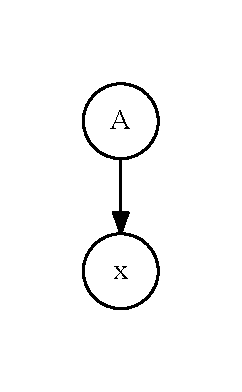
\includegraphics[width=2cm]{pictures/tree1.pdf}
		\caption{The derivation tree of the height $h = 1$ for the string $x = l(\pi)$.}
		\label{tree1}
	\end{figure}
	
	\textbf{Inductive step}: Assume that the statement of the lemma holds for any $k \leq (p - 1)$ and show that it also holds for $k = p$ where $p \geq 2$. For any $i, j$ and for any non-terminal $A \in N$, $$A \in a^{(p)}_{i,j} \text{ iff } A \in a^{(p-1)}_{i,j} \text{ or } A \in (a^{(p-1)} \times a^{(p-1)})_{i,j},$$ since $$a^{(p)} = a^{(p-1)} \cup (a^{(p-1)} \times a^{(p-1)}).$$
	
	Let $A \in a^{(p-1)}_{i,j}$. By the inductive hypothesis, $A \in a^{(p-1)}_{i,j}$ iff $(i,j) \in R_A$ and there exists $i \pi j$, such that there is a derivation tree of the height $h \leq (p-1)$ for the string $l(\pi)$ and a context-free grammar $G_A = (N,\Sigma,P,A)$. The statement of the lemma holds for $k = p$, since the height $h$ of this tree is also less than or equal to $p$.
	
	Let $A \in (a^{(p-1)} \times a^{(p-1)})_{i,j}$. By the definition of the binary operation $(\cdot)$ on arbitrary subsets, $A \in (a^{(p-1)} \times a^{(p-1)})_{i,j}$ iff there are $r$, $B \in a^{(p-1)}_{i,r}$ and $C \in a^{(p-1)}_{r,j}$, such that $(A \rightarrow B C) \in P$. Hence, by the inductive hypothesis, there are $i \pi_1 r$ and $r \pi_2 j$, such that $(i,r) \in R_B$ and $(r,j) \in R_C$, and there are the derivation trees $T_B$ and $T_C$ of heights $h_1 \leq (p-1)$ and $h_2 \leq (p-1)$ for the strings $w_1 = l(\pi_1)$, $w_2 = l(\pi_2)$ and the context-free grammars $G_B$, $G_C$ respectively. Thus, the concatenation of paths $\pi_1$ and $\pi_2$ is $i \pi j$, where $(i,j) \in R_A$ and there is a derivation tree of the height $h = 1 + max(h_1, h_2)$, shown in Figure~\ref{tree2}, for the string $w = l(\pi)$ and a context-free grammar $G_A$.
	
	\begin{figure}[h!]
		\centering
		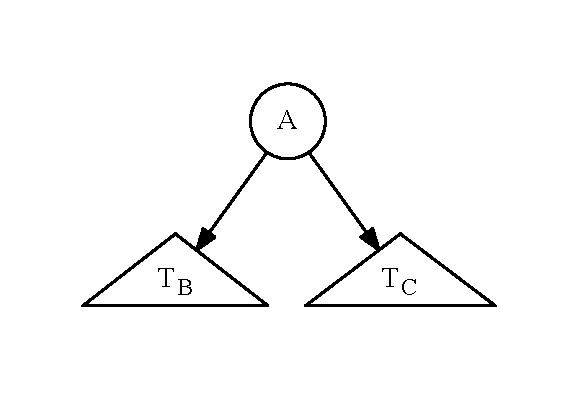
\includegraphics[width=5cm]{pictures/tree2.pdf}
		\caption{The derivation tree of the height $h = 1 + max(h_1, h_2)$ for the string $w = l(\pi)$, where $T_B$ and $T_C$ are the derivation trees for strings $w_1$ and $w_2$ respectively.}
		\label{tree2}
	\end{figure}
	
	The statement of the lemma holds for $k = p$, since the height $h = 1 + max(h_1, h_2) \leq p$. This completes the proof of the lemma.
\end{proof}